\documentclass[aspectratio=169,10pt]{beamer}

% Slide deck for orbit_transfer/orbit_network: what the Braik-Ross orbital-
% network framing says about the four certified min-time costate catalogs.
% Every number is read from results/network_summary.txt and the
% stability_cost_study output; figures from slides/make_slide_figures.m.
% Companion to doc/orbit_network_note.tex.

\usetheme{default}
\usecolortheme{seahorse}
\setbeamertemplate{navigation symbols}{}
\setbeamertemplate{footline}[frame number]
\setbeamertemplate{itemize items}[circle]
\setbeamercolor{frametitle}{fg=black!85,bg=blue!8}
\setbeamerfont{frametitle}{size=\normalsize,series=\bfseries}
\setbeamercolor{block title}{fg=white,bg=blue!55!black}
\setbeamercolor{block body}{bg=blue!5}
\setlength{\leftmargini}{1.2em}
\usepackage{booktabs,amsmath,amssymb}
\newcommand{\key}[1]{\texttt{#1}}
\graphicspath{{figures/}}

\title{A Low-Thrust Orbital Network over the Costate Catalogs}
\subtitle{What the Braik--Ross ``orbital network'' framing says about our certified min-time transfers}
\author{Michael Casey}
\date{November 2026}

\begin{document}

\begin{frame}
  \titlepage
\end{frame}

% ------------------------------------------------------------------ 1
\begin{frame}{The question: does the network view, or orbit stability, say anything about transfers we already hold?}
  \small
  \begin{columns}[T]
    \begin{column}{0.5\textwidth}
      \textbf{Braik and Ross (arXiv 2605.31543)}
      \begin{itemize}
        \item 13 planar Earth--Moon periodic orbits on one Jacobi level
        \item edge score = overlap of reachable sets under heading-change impulses
        \item read hubs, relay orbits, budget-dependent connectivity stages
        \item stability reading: unstable orbits share a chaotic sea and connect cheaply; stable ones sit inside tori
      \end{itemize}
    \end{column}
    \begin{column}{0.5\textwidth}
      \textbf{What we lifted it onto}
      \begin{itemize}
        \item four min-time costate catalogs: spatial CR3BP, continuous thrust with mass loss
        \item edge cost = certified min-time extremals (multiple shooting, conjugate test, hypothesis gates)
        \item a $6\times6$ departure/arrival phasing grid per sheet, 11 thrust rungs from 15~N to 0.5~N
        \item \textbf{no proxies, no new solves}: data only
      \end{itemize}
    \end{column}
  \end{columns}
  \vspace{8pt}
  \begin{block}{Two questions}
    (1) Does departure instability predict cheaper or hardier transfers, beyond the energy gap?\\
    (2) What does the catalog look like as a network: coverage against thrust and time, relays, closure down the ladder?
  \end{block}
\end{frame}

% ------------------------------------------------------------------ 2
\begin{frame}{The data: 56 certified sheets over 18 orbits, no new solves}
  \begin{columns}[T]
    \begin{column}{0.55\textwidth}
      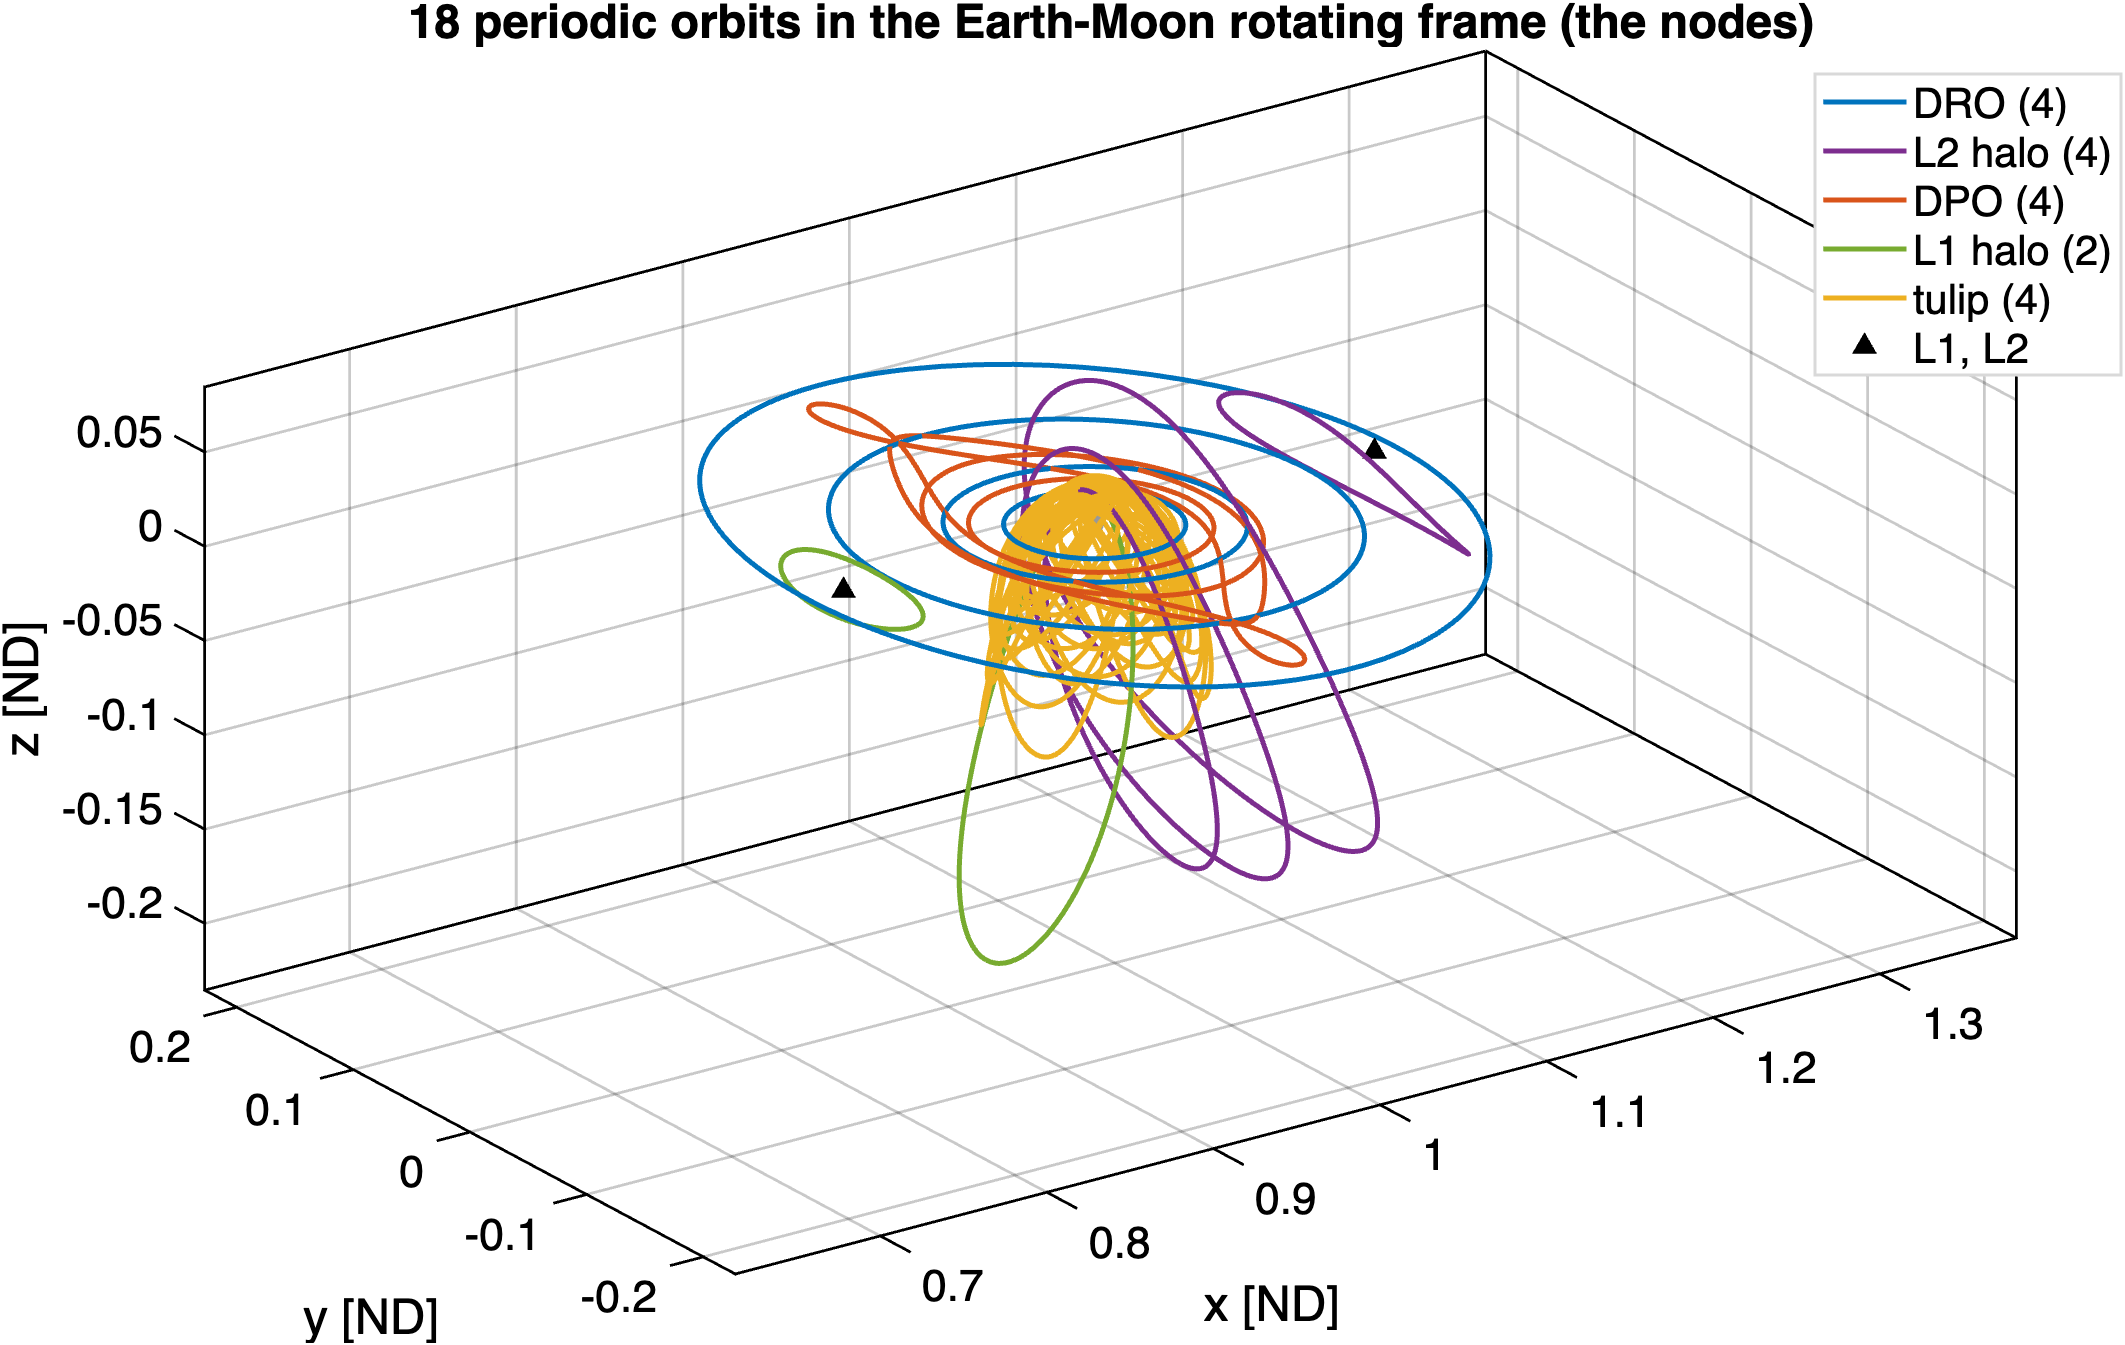
\includegraphics[width=\textwidth]{nodes_3d.png}\\
      {\footnotesize Rotating frame, ND = Earth--Moon distance. Triangles: L1, L2.}
    \end{column}
    \begin{column}{0.45\textwidth}
      \footnotesize
      \setlength\tabcolsep{3pt}
      \begin{tabular}{@{}lr@{}}
        \toprule
        catalog & sheets \\
        \midrule
        DRO $\tau=0.5,1,2,3$ $\to$ tulip $N_p=5,7,9,12$ & 16 \\
        L2 halo $\tau=1.75,2.2,2.8,3.4$ $\to$ tulips & 16 \\
        DPO $\tau=1,2,3,4$ $\to$ tulips & 16 \\
        L1 halo $\tau=1.80,2.74$ $\to$ the L2 halos & 8 \\
        \bottomrule
      \end{tabular}
      \vspace{6pt}
      \begin{itemize}
        \item a sheet = one (departure, arrival) pair; $6\times6$ phasing cells on each of 11 rungs
        \item a cell is \textbf{accepted} when solved, conjugate-pass, and positive on the three hypothesis gates ($\min|\lambda_v|$, $Q_{mt}$, $\dim S=1$)
        \item every count, minimum, plane and route is over accepted cells: 1118 at 1~N, 898 at 0.5~N
        \item an unaccepted cell is unresolved, never a proven infeasibility
      \end{itemize}
    \end{column}
  \end{columns}
\end{frame}

% ------------------------------------------------------------------ 3
\begin{frame}{A relay can never beat the unrestricted optimum}
  \begin{block}{Lemma (set inclusion)}
    Let $\mathcal F_{AB}$ be the feasible trajectories of the $A\to B$ optimal control problem, mass included, and
    $\mathcal R_{ACB}\subseteq\mathcal F_{AB}$ those that pass through relay orbit $C$ with compatible full states. Then
    $\displaystyle\inf_{\mathcal F_{AB}} J \le \inf_{\mathcal R_{ACB}} J$.
  \end{block}
  \vspace{4pt}
  \begin{itemize}
    \setlength\itemsep{5pt}
    \item Their ``multileg advantage'' is relative to a restricted direct-maneuver class, not to the global optimum.
    \item A relay witness below the thrust where our direct branch stops would be \emph{another feasible transfer}: it diagnoses the branch or the search, not a global barrier.
    \item Legs solved from $m_0$ compose without a new solve: scale leg 2's thrust and mass by $q = m_1/m_0 \le 1$. Same path, thrust bound respected. Feasible, not thereby optimal.
    \item So the data can show \textbf{where relays close}, never that a relay is cheaper than the direct transfer.
  \end{itemize}
\end{frame}

% ------------------------------------------------------------------ 4
\begin{frame}{The network at 1 N: all 56 edges carry a certified transfer, and all 56 still do at 0.5 N}
  \begin{columns}[T]
    \begin{column}{0.66\textwidth}
      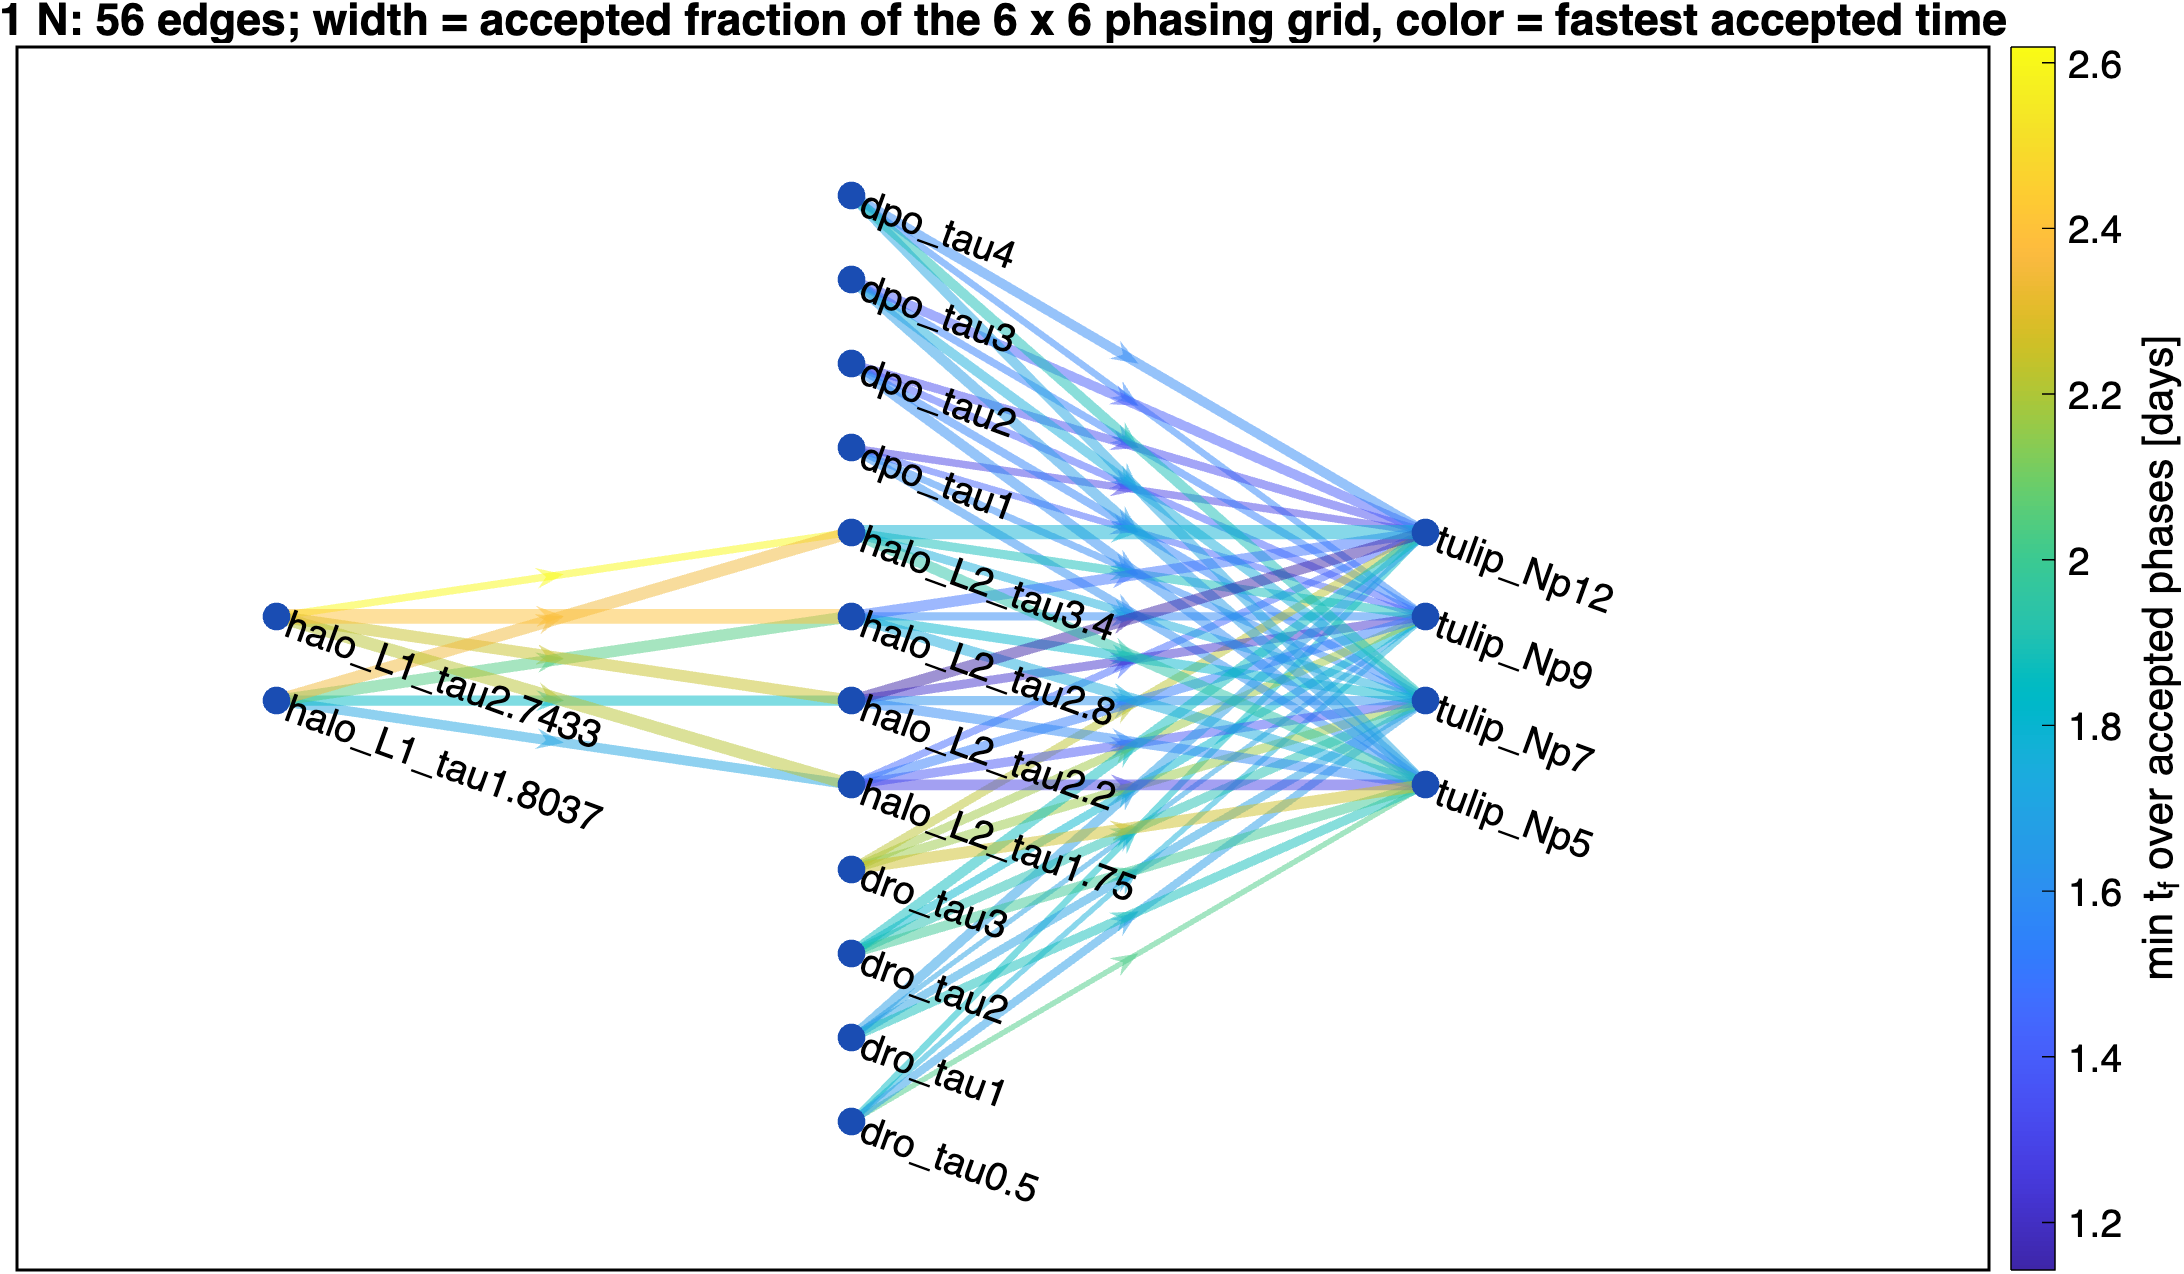
\includegraphics[width=\textwidth]{network_graph_1N.png}
    \end{column}
    \begin{column}{0.34\textwidth}
      \footnotesize
      \begin{itemize}
        \item 18 nodes, 56 directed edges = the sheets
        \item every edge has an accepted cell at 1~N and at 0.5~N; the ``lowest accepted rung'' is where the ladder stopped with a witness, not a floor
        \item fastest at 1~N: L2 halo $\tau=2.2$ $\to$ tulip $N_p=12$ (1.14~d), $N_p=9$ (1.22~d)
        \item slowest: L1 halo $\tau=2.74$ $\to$ L2 halo $\tau=3.4$ (2.62~d)
        \item strengths are descriptive only: tulips have 12 in-edges, L2 halos 2 in and 4 out, everything else 4 out. The topology is the catalog's.
      \end{itemize}
    \end{column}
  \end{columns}
\end{frame}

% ------------------------------------------------------------------ 5
\begin{frame}{Thrust bound against time cap: at 1 N every direct pair is covered under 2.75 days}
  \begin{columns}[T]
    \begin{column}{0.6\textwidth}
      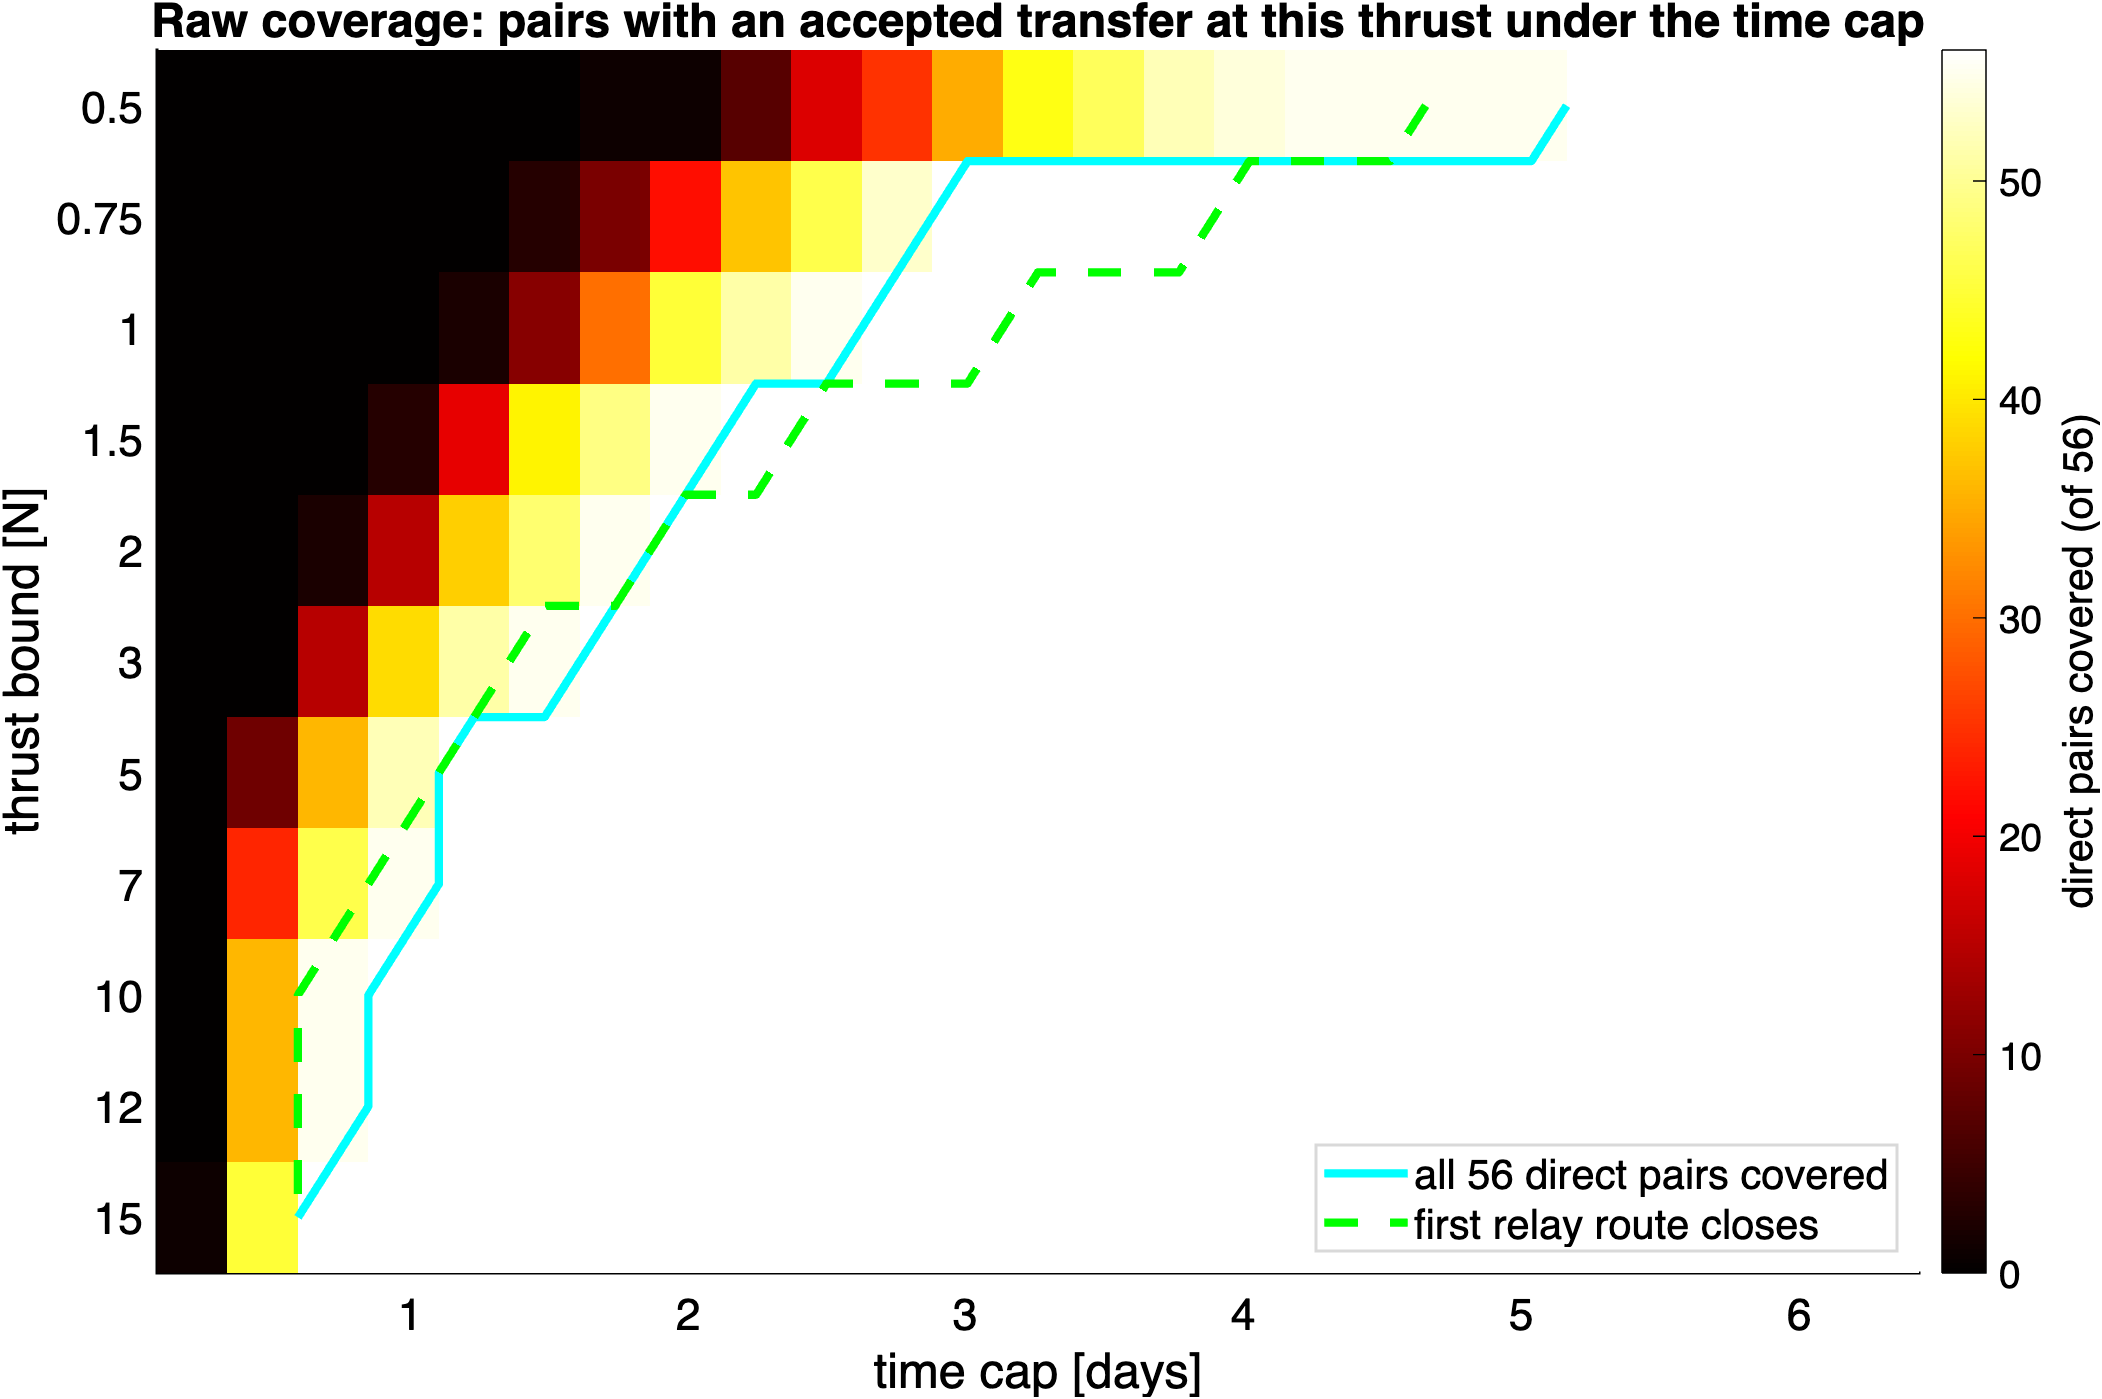
\includegraphics[width=\textwidth]{accessibility_plane_raw.png}
    \end{column}
    \begin{column}{0.4\textwidth}
      \footnotesize
      \begin{itemize}
        \item thrust is a capability axis for one spacecraft, not a budget: 11 rungs $\times$ 25 caps (0.22 to 6.3~d)
        \item raw coverage = pairs with an accepted cell \emph{at} that rung under the cap
        \item the known-feasible envelope (accepted at that rung \emph{or any lower one}) exceeds raw at only 12~N and 3~N, by one pair each
        \item cyan: all 56 direct pairs; green: the first phase-compatible relay route. Diagnostics, not stages.
        \item the first relay closes \emph{before} the last direct pair at 12, 10, 7, 3 and 0.5~N; after it at 1.5, 1 and 0.75~N
      \end{itemize}
    \end{column}
  \end{columns}
\end{frame}

% ------------------------------------------------------------------ 6
\begin{frame}{Down the ladder the families separate: DRO and DPO lose half their phasings, L1 halos keep most}
  \begin{columns}[T]
    \begin{column}{0.6\textwidth}
      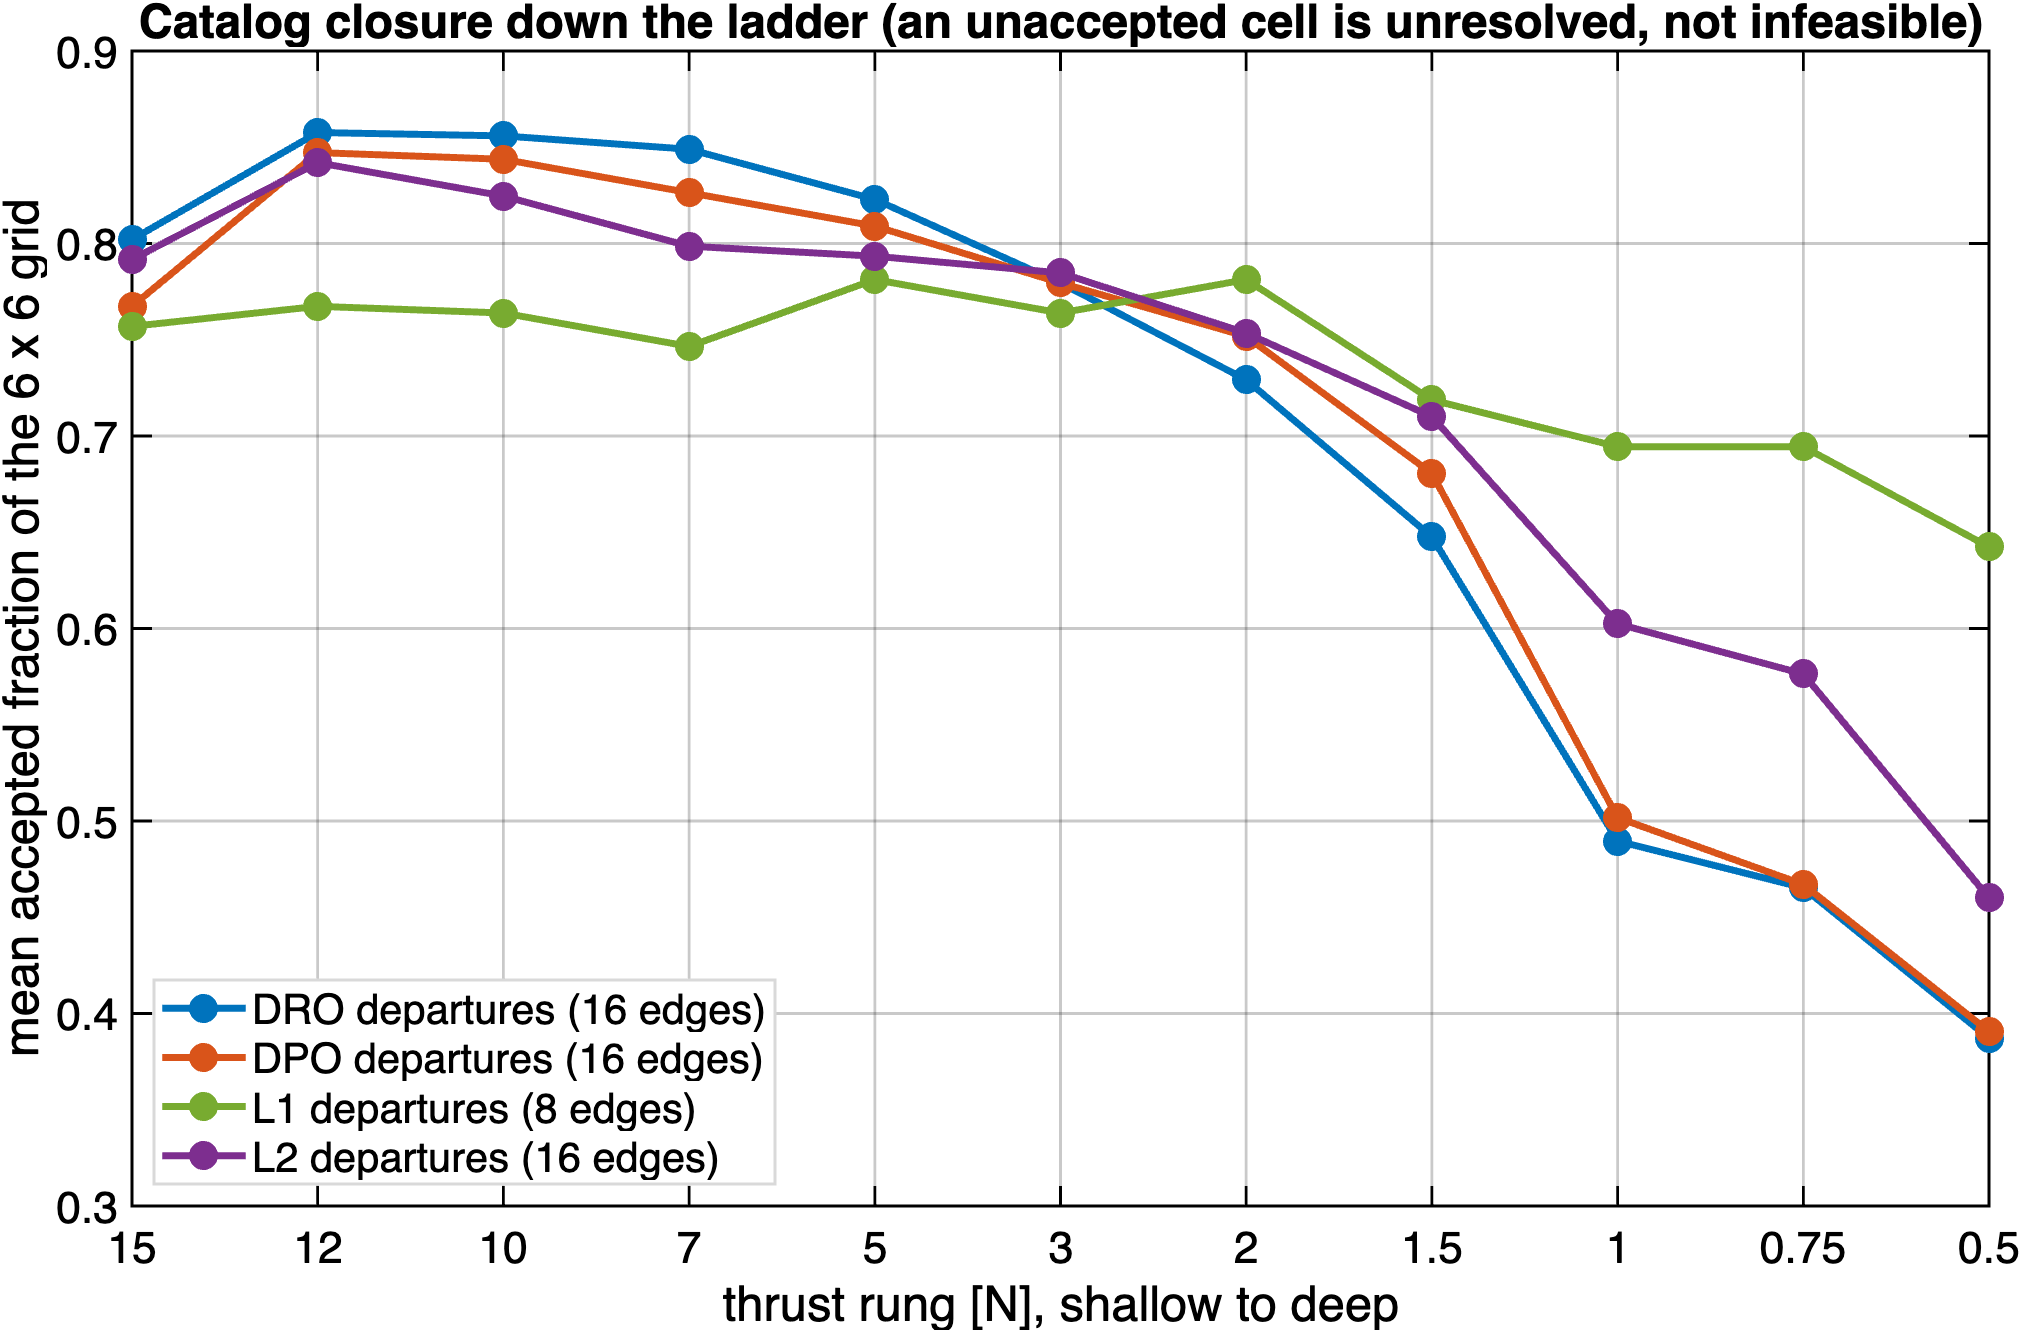
\includegraphics[width=\textwidth]{ladder_closure.png}
    \end{column}
    \begin{column}{0.4\textwidth}
      \footnotesize
      mean accepted fraction of the $6\times6$ grid
      \vspace{3pt}

      \begin{tabular}{@{}lcc@{}}
        \toprule
        departures & 12 N & 0.5 N \\
        \midrule
        DRO (all stable)          & 0.86 & 0.39 \\
        DPO (3 of 4 unstable)     & 0.85 & 0.39 \\
        L2 halo (3 of 4 unstable) & 0.84 & 0.46 \\
        L1 halo (both unstable)   & 0.77 & 0.64 \\
        \bottomrule
      \end{tabular}
      \vspace{6pt}
      \begin{itemize}
        \item the 15~N dip is ladder coverage: the starting rung holds fewer solved cells than 12~N
        \item solved sets nest between 1~N and 0.5~N; accepted sets do not (4 cells accepted at 0.5~N, refuted at 1~N)
        \item this is where a stable/unstable contrast shows: by family, not in the sheet regression
      \end{itemize}
    \end{column}
  \end{columns}
\end{frame}

% ------------------------------------------------------------------ 7
\begin{frame}{The one relay in the data closes for all 8 pairs down to 0.5 N, always with a zero-wait phasing}
  \begin{columns}[T]
    \begin{column}{0.56\textwidth}
      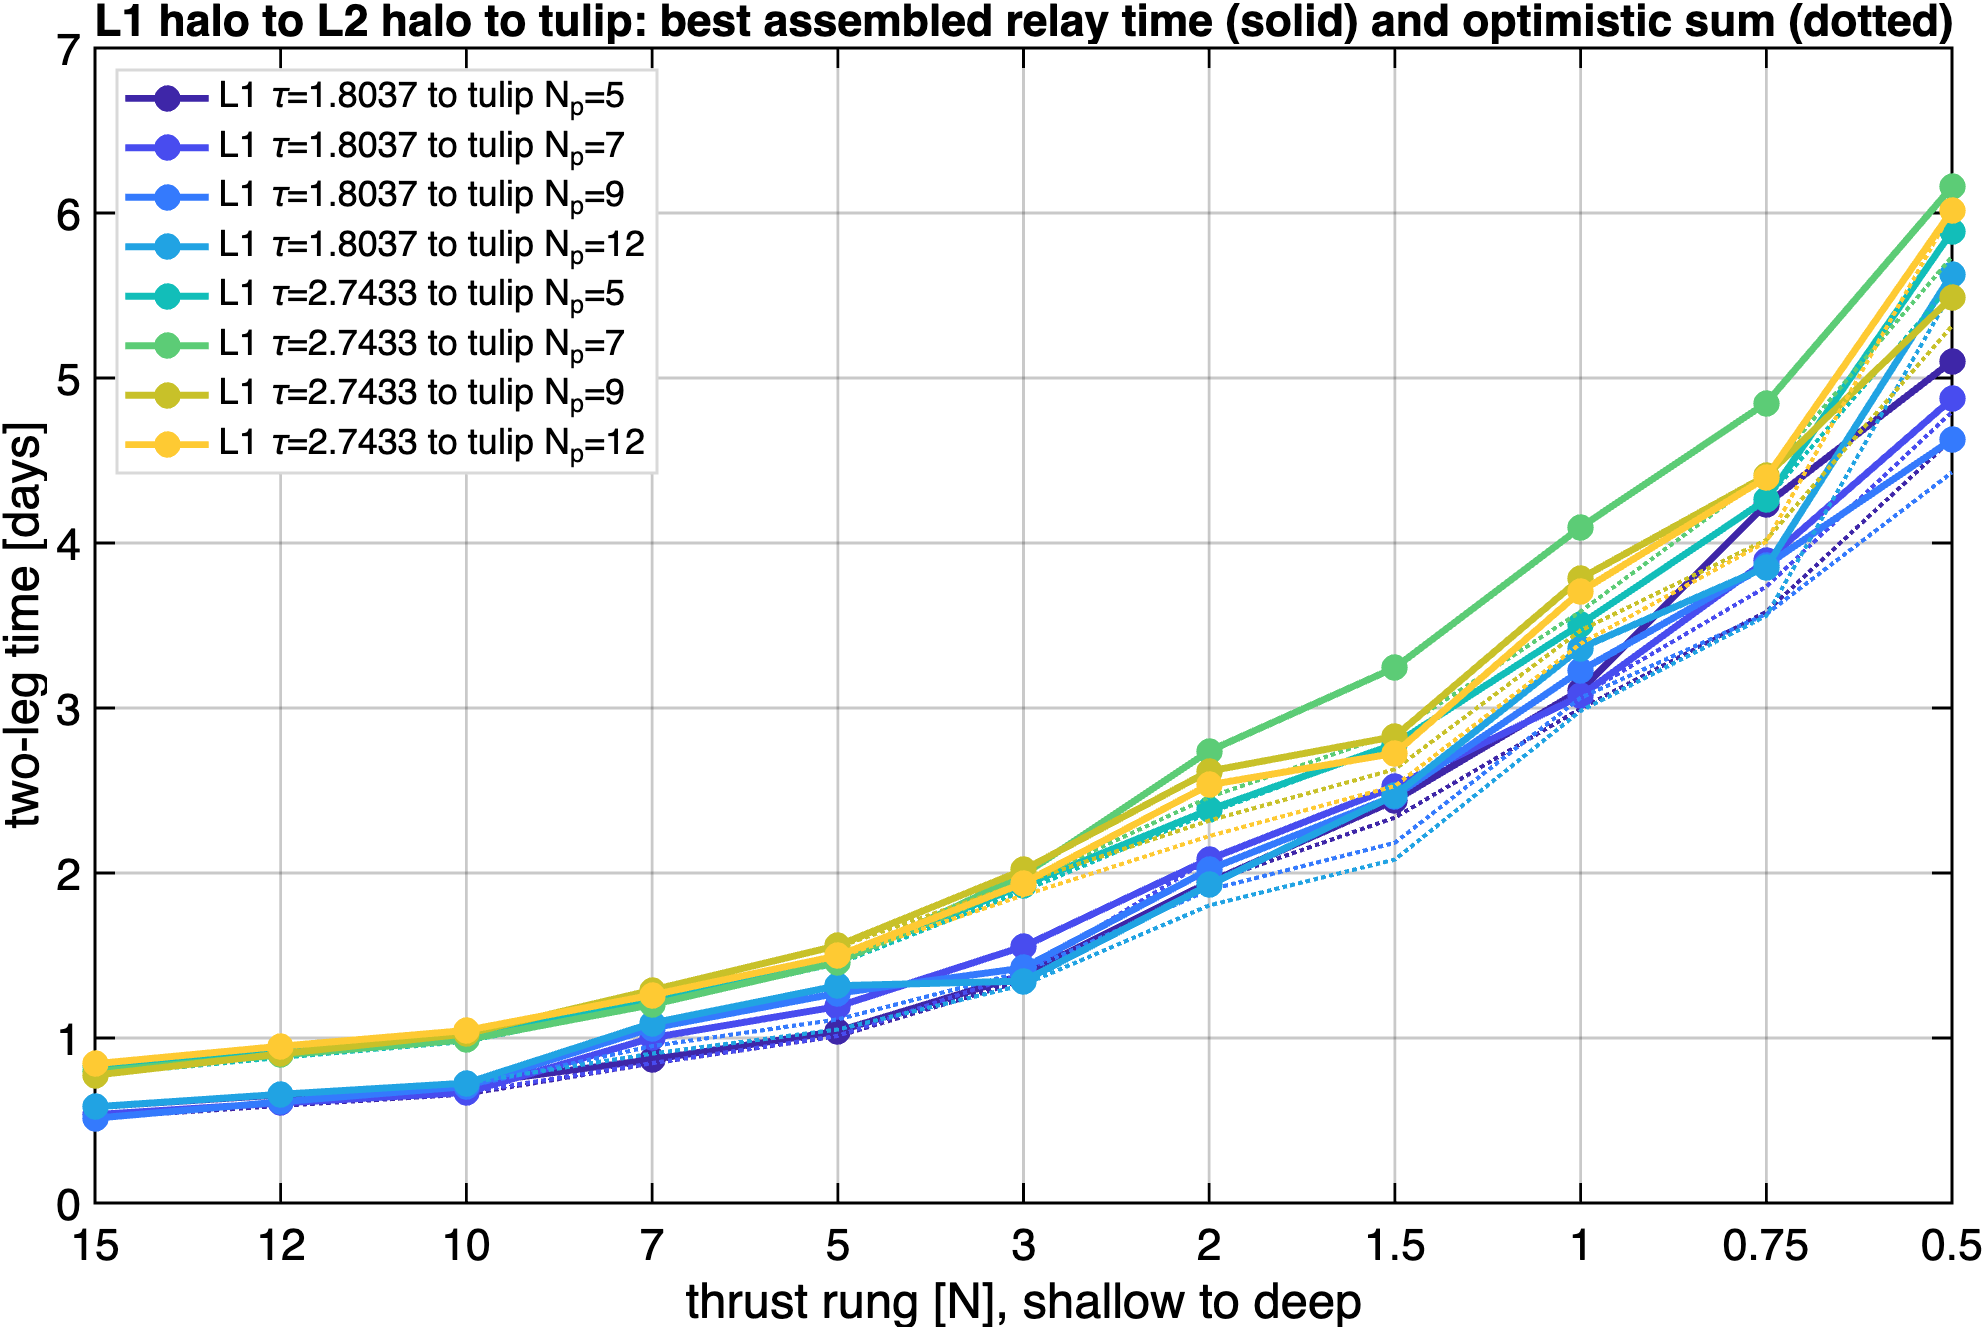
\includegraphics[width=\textwidth]{relay_closure.png}
    \end{column}
    \begin{column}{0.44\textwidth}
      \footnotesize
      L1 halo $\to$ L2 halo $\to$ tulip: $2\times4\times4 = 32$ routes over 8 pairs. Phase-compatible assembled time over accepted cells,
      \[
        t_{\rm route}=\min_{(a,b),(c,d)}\big[\,t_1 + T_C\,\mathrm{mod}(s_{D2}-s_{A1},1) + t_2\,\big];
      \]
      the optimistic sum $\min t_1+\min t_2$ is only a lower bound.
      \begin{itemize}
        \item all 352 closed (route, rung) pairs find a zero-wait pairing; 7 of 32 routes hit the sum at 1~N
        \item best relay at 1~N: L2 halo $\tau=1.75$ for 5 pairs, $\tau=2.2$ for 3; $\tau=2.8$ and $3.4$ never
        \item route times at 1~N: 3.07 to 4.10~d
        \item relay-versus-direct cost is untestable here: no direct L1 halo $\to$ tulip edge exists
      \end{itemize}
    \end{column}
  \end{columns}
\end{frame}

% ------------------------------------------------------------------ 8
\begin{frame}{Stability versus cost: departure instability adds nothing detectable beyond the Jacobi gap}
  \begin{columns}[T]
    \begin{column}{0.6\textwidth}
      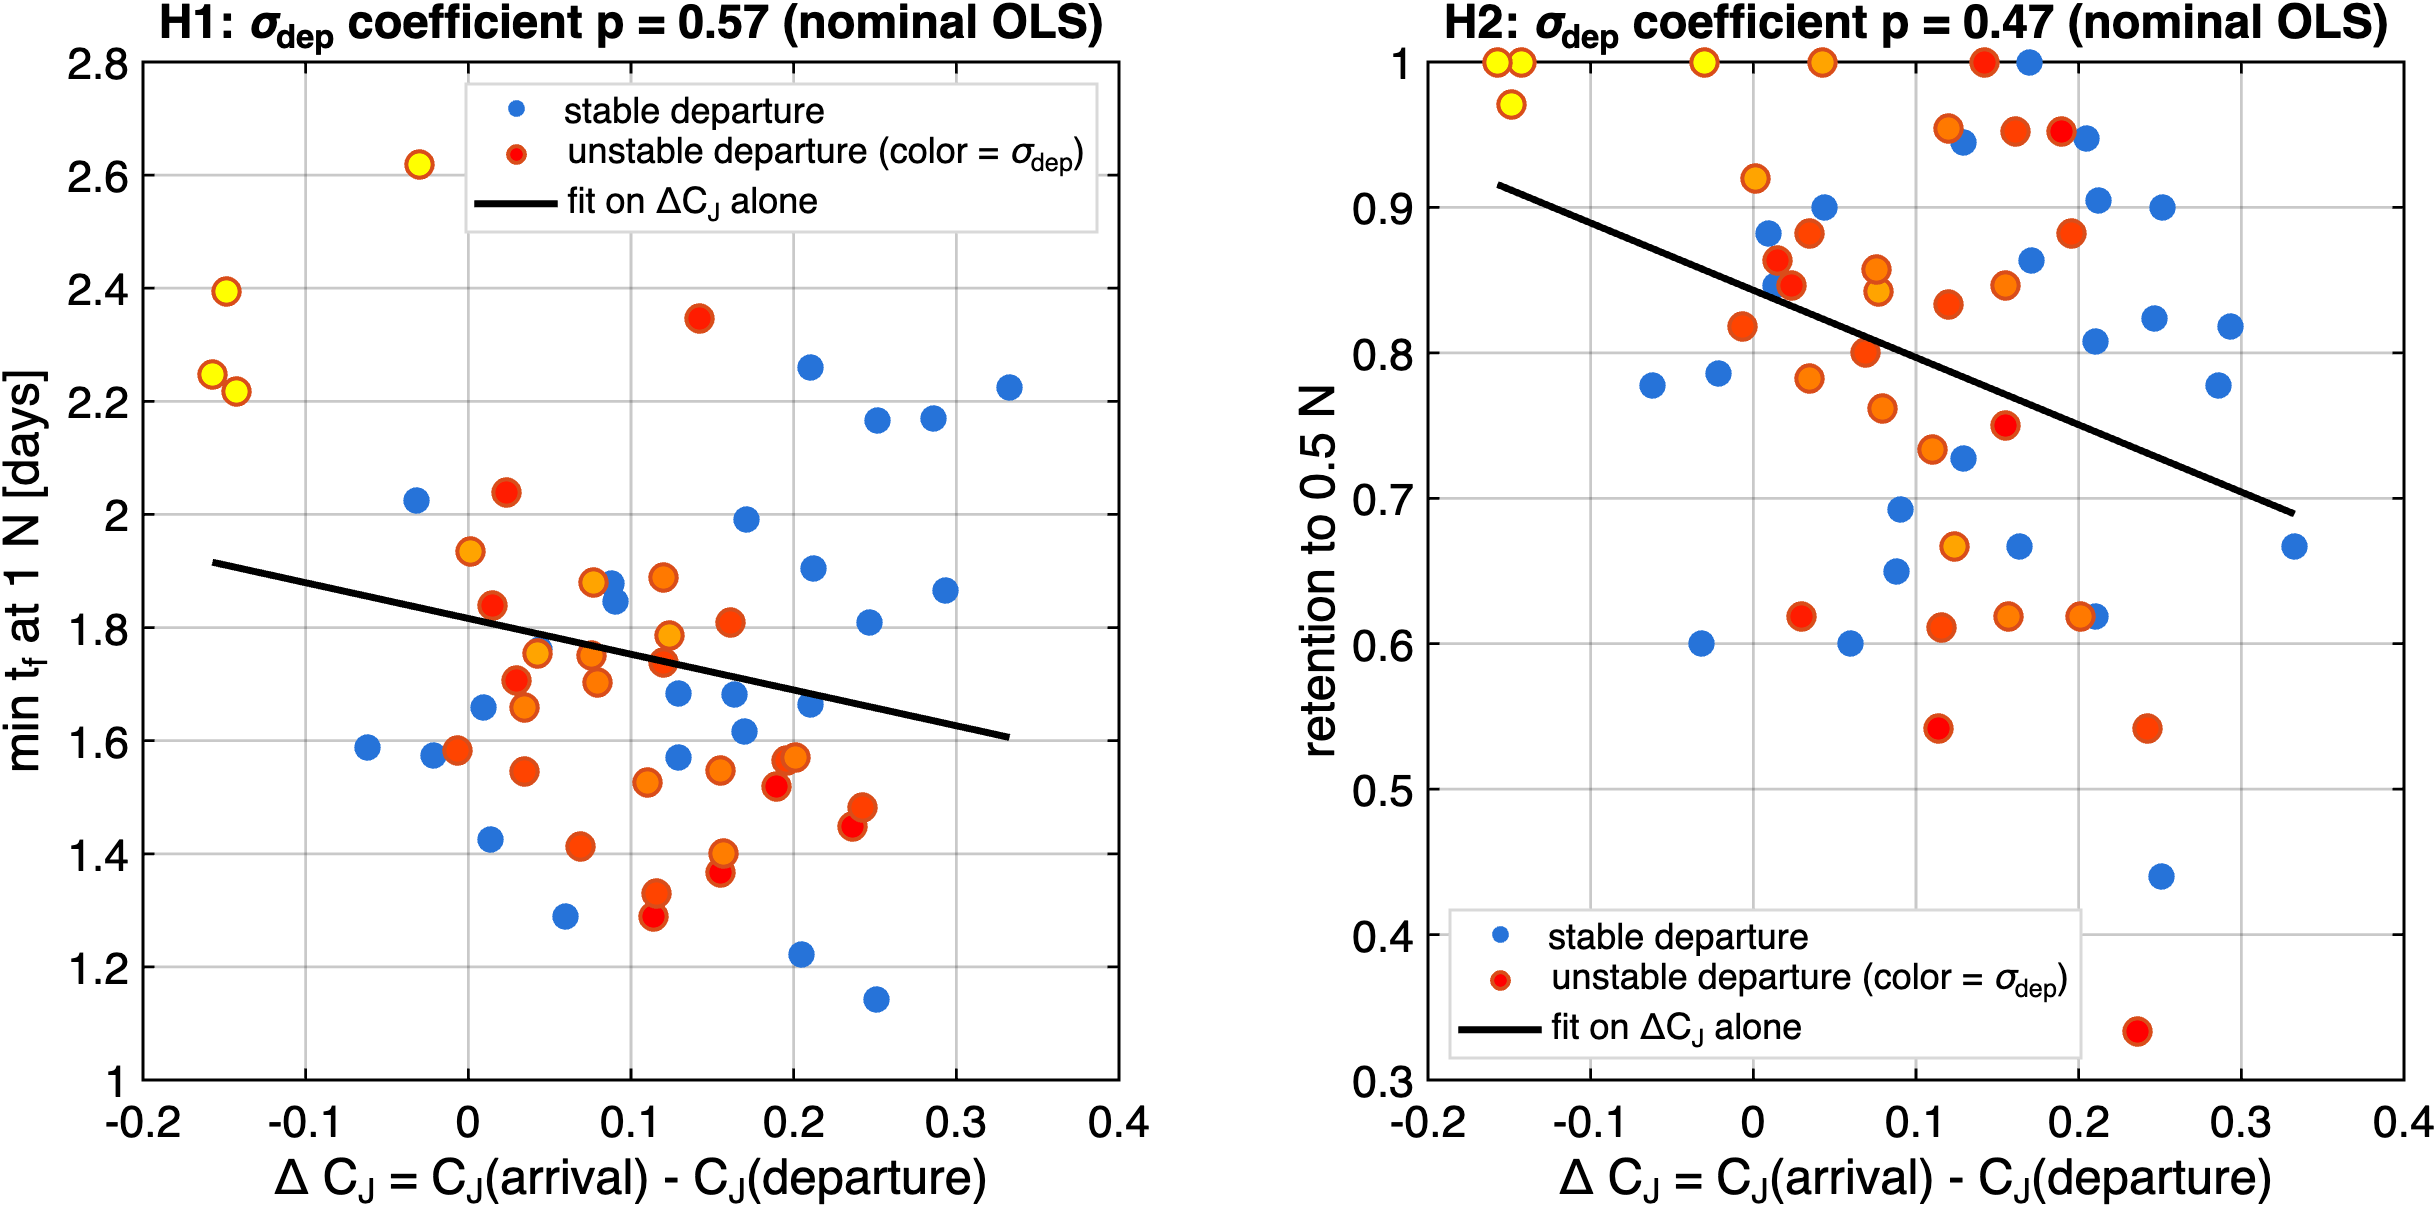
\includegraphics[width=\textwidth]{stability_cost.png}
    \end{column}
    \begin{column}{0.4\textwidth}
      \footnotesize
      $\sigma=\ln|\lambda|_{\max}/T$ from the monodromy matrix, 0 when stable. 24 stable-departure sheets, 32 unstable.
      Nested OLS: M0 on $\Delta C_J$; M1 adds $\sigma_{\rm dep},\sigma_{\rm arr}$.
      \vspace{3pt}

      \setlength\tabcolsep{4pt}
      \begin{tabular}{@{}lcc@{}}
        \toprule
        $\sigma_{\rm dep}$ coeff. & $t_f$ at 1 N & retention \\
        \midrule
        estimate       & 0.027 & 0.019 \\
        95\% CI        & $[-0.07,0.12]$ & $[-0.03,0.07]$ \\
        $p$ (nominal)  & 0.57 & 0.47 \\
        paper predicts & negative & positive \\
        \bottomrule
      \end{tabular}
      \vspace{5pt}
      \begin{itemize}
        \item H1, H2: \textbf{NOT DETECTED} (nominal OLS)
        \item the joint $F$ for $t_f$ is significant ($p=10^{-4}$) but rides on $\sigma_{\rm arr}$, which varies only on the 8 halo-to-halo sheets
        \item sheets share nodes (14 departures, 8 arrivals); nonsignificance is not equivalence; 1~N is far above the 70~mN regime
      \end{itemize}
    \end{column}
  \end{columns}
\end{frame}

% ------------------------------------------------------------------ 9
\begin{frame}{What we deliberately did not claim}
  \begin{itemize}
    \setlength\itemsep{7pt}
    \item \textbf{No relay-versus-direct cost.} The lemma says the unrestricted optimum is never above a relay's; the data has no pair with both a direct edge and a relay route.
    \item \textbf{No thrust floors.} A lowest accepted rung bounds nothing below it; the ladder stopped there with a witness.
    \item \textbf{No connectivity stages.} The cyan and green contours are diagnostics on sampled caps.
    \item \textbf{No hubs or betweenness.} Only the L2 halos have both in- and out-edges, so any centrality restates the catalog.
    \item \textbf{No reversed transfers.} The x-axis symmetry maps a thrusting arc to a thrusting arc of a \emph{mass-gain} model. The reversed graph (112 edges, one strongly connected component, 306 of 306 ordered pairs) is geometry only, labelled HYPOTHETICAL, off by default.
    \item \textbf{No ``no effect''.} NOT DETECTED at sheet level with nominal $p$-values, far from the 70~mN operating point and the wall between 0.09 and 0.067~N where the DRO deep continuation stalls.
  \end{itemize}
\end{frame}

% ------------------------------------------------------------------ 10
\begin{frame}{Next: the legs campaign, and Earth $\to$ DRO $\to$ tulip hopping}
  \small
  \begin{columns}[T]
    \begin{column}{0.5\textwidth}
      \textbf{Legs that make the comparison testable}
      \begin{itemize}
        \item DRO $\to$ DPO and DRO $\to$ L2 halo, carried toward 70~mN
        \item then DRO $\to$ tulip is the first pair with both a direct edge and a relay route
        \item a relay witness below the direct continuation's wall is a new feasible transfer: it speaks to that continuation, not to a barrier
        \item the present data ranks L2-halo relay candidates ($\tau=1.75$, $2.2$) but says nothing about DRO $\to$ L2 leg costs
      \end{itemize}
    \end{column}
    \begin{column}{0.5\textwidth}
      \textbf{Getting to the DRO in the first place}
      \begin{itemize}
        \item the catalogs never say how a spacecraft reaches a DRO
        \item nearest existing piece: the GTO $\to$ tulip min-time catalog (deliverable 7, 16 orientation sheets, deep rungs 3 to 1~N open)
        \item a GTO $\to$ DRO leg makes GTO $\to$ tulip a second pair with a direct edge and a relay route
        \item so Earth $\to$ DRO $\to$ tulip hopping is a legs-campaign candidate; the data does not rank it against the others
      \end{itemize}
    \end{column}
  \end{columns}
  \vspace{8pt}
  Mechanics: new ladder jobs on the shared engine (\key{thrust\_ladder\_library}) plus the GTO catalog in the loader.
\end{frame}

% ------------------------------------------------------------------ 11
\begin{frame}{Where it lives and how it was checked}
  \small
  \key{orbit\_transfer/orbit\_network/}
  \begin{itemize}
    \setlength\itemsep{4pt}
    \item \key{stability\_cost\_study.m} and \key{orbit\_network\_study.m}: numbered sections, every condition computed in-script with PASS/FAIL; gates P1--P7 and G1--G5 all pass
    \item \key{lib/}: edge tables, graph (attributes read from \key{G.Edges}, since MATLAB sorts edges), accessibility planes, phase-compatible relay closure, mirror state and symmetry residual, nested-OLS partial $F$ with CIs
    \item \key{tests/run\_tests}: 4 of 4, including the headless pipeline with the hypothetical and cap-limited runs
    \item \key{results/network\_summary.txt}: every number the note and these slides cite, printed by the script
    \item \key{doc/orbit\_network\_note.tex}: 7 pages; \key{slides/make\_slide\_figures.m} redraws these figures from the same workspaces
    \item \key{reviews/}: GPT-6 Astra pre-build review (15 findings, all accepted and recorded) and the whole-branch final review
  \end{itemize}
  \vspace{4pt}
  Data traps caught on the way: \key{conj\_pass} stores $-1$ for ``not run'' (test $==1$); accepted sets are not nested between rungs; every stored $x_0$ lies on the symmetry plane, so the mirror check is made off-plane.
\end{frame}

\end{document}
